\chapter{Humanoid Posture Generation on non-Euclidean Manifolds}

\section{abstract}
We present a reformulation of the posture generation problem that encompasses non-Euclidean manifolds. 
Such a formulation allows a more elegant mathematical description of the constraints, which we exemplify through some scenarios in the simulation results section.
In our previous work, the posture generation problem is formulated as a non-linear optimization program with constraints expressed only through Euclidean manifolds; we solve the latter problem using on-the-shelf solvers.
Instead, we decided to implement a new SQP solver that is most suited to non-Euclidean manifolds structural objects.
By doing so, we have a better mastering in the way to tune and specialize our SQP solver for robotic problems.


\section{Introduction}
\label{sec:Intro}
Computing robot configurations to meet the requirements of a given set of tasks, within a viable state, is a recurrent problem whose complexity grows with that of the robot. In this paper, we are interested in the following generalized inverse kinematics problem: we search a configuration for which the robot fulfills tasks under constraints of joint limits, auto-collision and non-desired collision avoidance, balance, torque limits, etc. We coined it posture generation. Such a problem is encountered in both planning and control. In both cases, computation time and robustness are critical issues.

We have already proposed various implementations of the humanoid posture generation problem. All of our implementations formulate the problem as a non-linear optimization program to address multi-contact planning. In~\cite{escande:ras:2013}, the multi-contact planner explores the contact space using thousands of HRP-2 humanoid posture generator (PG) queries; we used the FSQP solver~\cite{cfsqp:manual}. In~\cite{bouyarmane:ar:2012}, the PG is extended to handle various humanoid robots and multiple agents, the solver used is IPOPT~\cite{wachter:mp:2006}. In~\cite{vaillant:humanoids:2014} the PG is extended to various contact models and used to generate multiple related postures at once. The latter work and the DRC participation revealed that re-planning on the fly is necessary and having a robust PG is crucial in many situations. Other works also make use of PG, e.g. in~\cite{hauser:humanoids:2005}\cite{Aristidou2009}.

Posture generation has been formulated as a problem over a Euclidean space. Robots variable may however be more naturally expressed over non-Euclidean manifolds. The archetypes for this are the rotation part of the root body for a humanoid robot, and ball joints, whose variables live in $SO(3)$. Some typical tasks are also naturally formulated on different manifolds. For example for making contact with any object that can be mapped on a sphere, the contact point position for this object can be parametrized in $S2$. Human shoulder can be elegantly parametrized on $S2\times\mathbb{R}$, as proposed in~\cite{Baerlocher}.

\begin{figure}[!tb]
\centering
  \centering
  \setlength\fboxsep{0pt}
  \setlength\fboxrule{1pt}
  \fbox{\includegraphics[width=.95\linewidth]{papers/Humanoids2015/figure/hrp4CubeOnSphere.png}}
\caption{HRP-4 carrying a 2-kg cube. Left: feet on a sphere, objective function is to maintain the cube at a given position. Right: right foot free to move on the floor, objective is to put the cube as far as possible in a given direction}
\label{fig:hrp4_cube}
\end{figure}

Formulating the problem over $\mathbb{R}^n$ leads either to discontinuities that can prevent the convergence of the optimization solver, or to cumbersome writing to specify that the variable is actually living on a manifold (see~\cite{bouyarmane:humanoids:2012}).

In this paper, we propose a new optimization solver able to work on generic smooth manifolds. We take inspiration from the approach used for unconstrained optimization on manifold~\cite{absil:book:2008} and adapt it to constrained optimization. To the best of our knowledge, constrained optimization on manifold has drawn few research for now. This is likely due to the fact that in most problems the only constraint is to be on the manifold. We are only aware of the work of Schulman~\emph{et al.}~\cite{Schulman2014}, where the authors explain the adaptation of their solver to work on $SE(3)$. This adaptation is however not valid for general manifolds without more care about hessian computation.

The second contribution of this paper is a Posture Generation framework developed to ease the writing of functions, so that the user can focus on the problem formulation without having to care about the tedious bookkeeping inherent to optimization problems of this size.

A background motivation for this work is to have our own optimization solver, instead of a black box. We will now be able to specialize the solver specifically to robotic problems, by leveraging modeling properties and approximations, for a gain in time and robustness. We also look forward to using this solver for problems with a varying number of constraints along the iterations (such as when complex collision constraints are considered).

The rest of the paper is organized in a classical way: we start with a bit of math to describe the foundations; then we introduce the PG~\emph{per se}, the problem formulation followed with illustration of successful generations. 

\newcommand{\reduce}[2]{\hspace{-#2pt} #1 \hspace{-#2pt}}

\section{Optimization on Manifolds}
\label{sec:1}
In this section, we describe a Sequential Quadratic Programming (SQP) approach~\cite{nocedal:book:2006} to solve the following non-linear constrained optimization program

\begin{align}
\label{eq:optim_problem}
  \minimize_{x \in \mathcal{M}} & \quad f(x)\\
  \text{subject to}&
  \begin{array}{rcl}
    {l} \leq & \reduce{c(x)}{8}& \leq {u} \nonumber
  \end{array}
\end{align}

where $\mathcal{M}$ is a $n$-dimensional smooth manifold and $c$ is a $m$-dimensional real-valued function.

\subsection{Representation problem}
When $\mathcal{M} = \mathbb{R}^n$, the problem~(\ref{eq:optim_problem}) is solved iteratively, starting from an initial guess $x_0$ and performing successive steps $x_{i+1} = x_i + {\bf p_i}$ where ${\bf p_i}$ is the increment found at the $i$-th iteration, until convergence is achieved. The strategy to compute ${\bf p_i}$ depends on the solver.

This classical scheme cannot be readily applied to optimization over non-Euclidean manifolds. First of all, only (a subset of) the real numbers can be stored in computers. To manipulate elements of $\mathcal{M}$ we need to choose a way to represent them in memory. This boils down to choosing a representation space $\mathbb{E} = \mathbb{R}^r$ (with $r \geq n$) and a map
\begin{equation}
  \psi\ :\ 
  \begin{array}{ccc}
    x & \reduce{\mapsto}{6} & \mathbf{x} \\
    \mathcal{M} & \reduce{\rightarrow}{6} & \mathbb{E}
  \end{array} \nonumber
\end{equation}
In the following, we identify $\mathcal{M}$ with the set $\psi(\mathcal{M}) \subseteq \mathbb{E}$.

With this representation, it is tempting to simply transform problem~(\ref{eq:optim_problem}) as an optimization over $\mathbb{R}^r$ with objective $f \circ \psi^{-1}$ and constraint $c \circ \psi^{-1}$, and solve it with a usual solver. But depending on the representation choice, one of the two following problems arises:\\
(i) $r=n$, then it is not possible in the general non-Euclidean case to find $\psi$ without derivative discontinuities. This can lead to critical convergence problems, \\
(ii) $r>n$, then most elements of $\mathbb{E}$ do not represent an element of $\mathcal{M}$ %($\psi(\mathcal{M})$ is a measure-zero subset of $\mathbb{E}$) 
and $\psi$ cannot be surjective. Constraints need to be added to force the solution on $\mathcal{M}$. As a result, the problem has more variables and constraints w.r.t (i). Moreover, the additional constraints are unlikely to be met along the iteration process (even if $x_i$ is an element of $\mathcal{M}$, $x_i+{\bf p_i}$ is likely not, as nothing enforces it). This means that in order to evaluate $f \circ \psi^{-1}$ and $c \circ \psi^{-1}$ at a given $x_i$, one has to project it on $\psi(\mathcal{M})$ first, effectively computing $f \circ \psi^{-1} \circ \pi$ and $c \circ \psi^{-1} \circ \pi$, where $\pi$ is the projection. The composition by $\pi$ is an additional burden in programming (see e.g. in~\cite{bouyarmane:humanoids:2012a}).

As a simple example, the set of 3D-rotations $SO(3)$ is a manifold of dimension $3$. The following (classical) choices can be made
\begin{itemize}
  \item Rotation matrix ${\bf R} \in \mathbb{R}^{3\times 3} \approx \mathbb{R}^9$, additional constraints: $\{{\bf R}^t{\bf R} = I\ ,\ \det({\bf R})=1\}$, projection by orthogonalization,
  \item Quaternion ${\bf q} \in \mathbb{R}^4$, additional constraints: $\{ \left\|{\bf q}\right\|=1\}$, projection $\pi({\bf x}) = {\bf x}/\left\|{\bf x}\right\|$,
  \item Euler angles ($\mathbb{E} = \mathbb{R}^3$), singularities when reaching gimbal lock.
\end{itemize}


\subsection{Local parametrization}
By definition, there is always, at a point $x$ of a smooth $n$-dimensional manifold $\mathcal{M}$, a smooth map $\varphi_x$ between an open set of $T_x\mathcal{M}$, the tangent space to $\mathcal{M}$ at $x$, and a neighborhood of $x$, with $\varphi_x(0) = x$. $T_x\mathcal{M}$ can be identified with $\mathbb{R}^n$. This gives us a local parametrization for $\mathcal{M}$. The driving idea of the optimization on manifolds is to change the parametrization at each iteration. Applying this idea, we can reformulate Problem~(\ref{eq:optim_problem}) around $x_i$ as
\begin{align}
\label{eq:local_problem}
\minimize_{{\bf z} \in T_{x_i}\mathcal{M}} & \quad f \circ \varphi_{x_i}({\bf z}) \\
  \text{subject to}&
  \begin{array}{rcl}
    {l} \leq & \reduce{c \circ \varphi_{x_i}({\bf z})}{8}& \leq {b} \nonumber
  \end{array}
\end{align} 
This is an optimization problem on $\mathbb{R}^n$. If we perform one iteration of a classical solver starting from ${\bf z_0} = 0$, we get an iterate ${\bf z_1}$, which corresponds to the iterate $x_{i+1} = \varphi_{x_i}({\bf z_1})$. We can then reformulate Problem~(\ref{eq:optim_problem}) around $x_{i+1}$, perform a new iteration and repeat the process until convergence.

\begin{figure}[!htb]
	\centering
  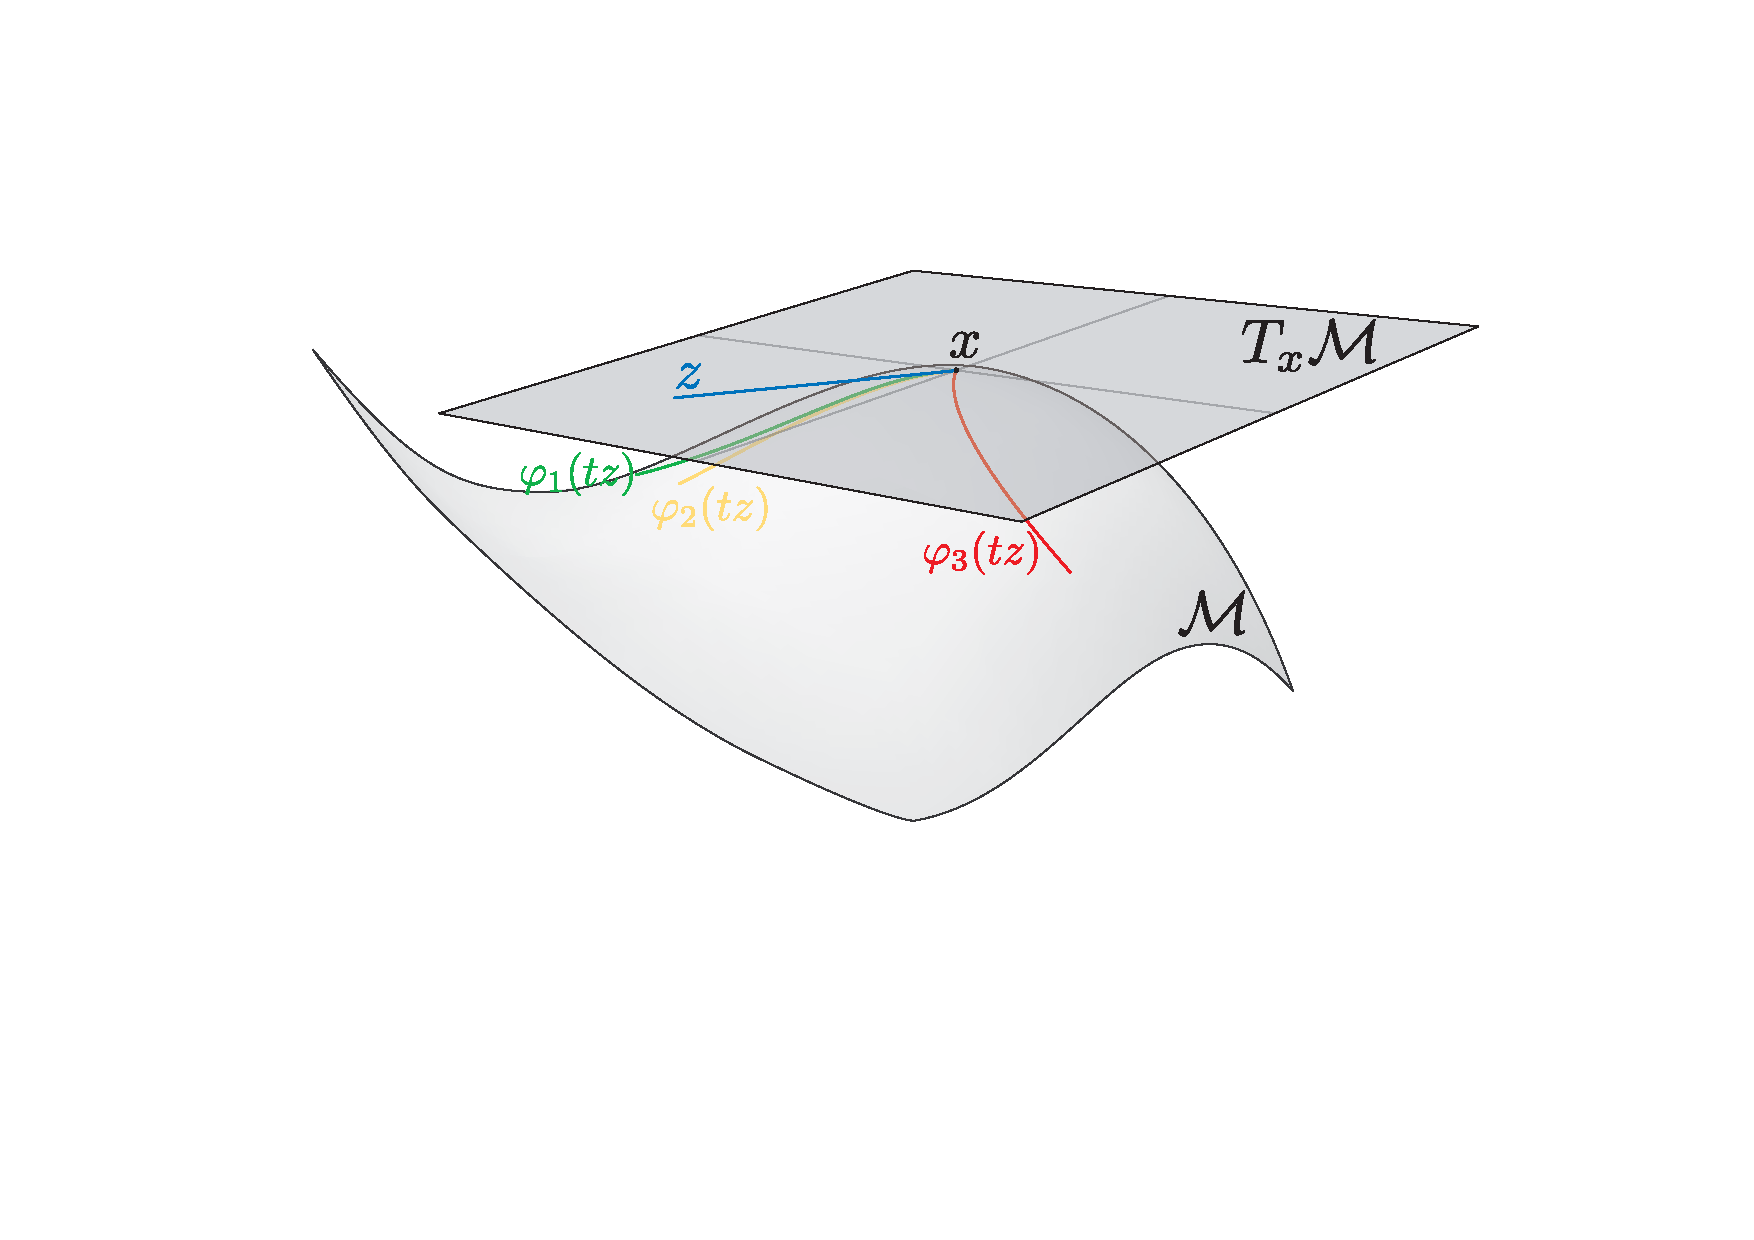
\includegraphics[width=.9\linewidth]{papers/Humanoids2015/figure/manifold.pdf}
    \caption{There are many possible choices for $\varphi_{x}$ but not all yield a curve $\varphi_{x}(t{\bf z})$ which is going in the same direction as ${\bf z}$: $\varphi_{1}$ and $\varphi_{2}$ are correct choices, $\varphi_{3}$ is not.}
	\label{fig:phimap}
\end{figure}


However, convergence cannot be achieved without care on the choice of $\varphi_{x_i}$: it must be such that for any ${\bf z}$, the curve $t \mapsto \varphi_{x_i}(tz)$ is tangent to ${\bf z}$, see Fig.~\ref{fig:phimap}, so that the update $x_{i+1} = \varphi_{x_i}({\bf z_1})$ is made in the direction given by ${\bf z_1}$.

The exponential map is a good theoretical candidate, but it is often impractical or expensive to compute. Depending on the manifold, cheaper maps can be chosen.

With the iterative formulation approach described above, we do not have any parametrization issue, do not need additional constraints, and have the minimum number of optimization parameters. But we still need a map $\psi$ and real space $\mathbb{E}$ to represent the $x_i$ and keep track of them in a global way. The ${\bf x_i}$ are guaranteed to be on $\mathcal{M}$ so we can choose a representation with $r>n$ where $\psi$ is singularity-free without any drawback.
Also, the programmer can write the function $f' = f \circ \psi^{-1}$ as if it was a function from $\mathbb{E}$ to $\mathbb{R}$ without the need to project on $\psi(\mathcal{M})$ first (same goes for $c' = c \circ \psi^{-1}$).
For example if $\mathcal{M} = SO(3)$ and $\mathbb{E} = \mathbb{R}^{3\times 3}$, ${\bf x_i}$ is automatically a rotation matrix and can be used directly as such when writing the function.

\subsection{Local SQP on manifolds}
We choose to adopt an SQP approach to solve our problem. We first define the Lagrangian function
\begin{equation}
  \mathcal{L}_x ({\bf z}, \lambda) = f\circ \varphi_x({\bf z}) - \lambda^T c \circ \varphi_x({\bf z})
\end{equation}
with $\lambda \in \mathbb{R}^m$ the vector of Lagrange multipliers, and note $H_k$ the Hessian matrix $\nabla_{zz}^2 \mathcal{L}_{x_k}$. Taking ${\bf z_0} = 0$, the first SQP step for Problem~(\ref{eq:local_problem}) is computed by solving the following quadratic program

\begin{align}
	\label{eq:SQPStep}
  \minimize_{\bf z \in \mathbb{R}^n } & \quad \frac{\partial f\circ \varphi_{x_k}}{\partial {\bf z}}(0)^T {\bf z } + \frac{1}{2} {\bf z }^T H_k{\bf z }\\
  \text{subject to}&
  \begin{array}{lr}
    \text{l} \leq c\circ \varphi_{x_k}(0) + \frac{\partial c\circ \varphi_{x_k}}{\partial {\bf z}}(0) {\bf z }\leq \text{u}\\
  \end{array} \nonumber
\end{align}

The basic SQP approach adapted to manifolds can be summarized as follows
\begin{enumerate}
	\item set $k=0$ and $x_k$ to the initial value
  \item compute ${\bf z}$ from Problem~(\ref{eq:SQPStep}) for current $x_k$
  \item set $x_k = \varphi_{x_k}({\bf z})$
	\item if convergence is not yet achieved go-to step 2
\end{enumerate}

Computations of function values and derivatives are based on the fact that $f \circ \varphi = f' \circ \psi \circ \varphi$ (and same for $c$), and
\begin{align}
  f'\ :\ 
  \begin{array}{ccc}
    \mathbb{E} & \reduce{\rightarrow}{6} & \mathbb{R}
  \end{array} \nonumber \\
	\psi \circ \varphi\ :\ 
  \begin{array}{ccc}
    \mathbb{R}^n & \reduce{\rightarrow}{6} & \mathbb{E}
  \end{array} \nonumber
\end{align}
are representable functions. The gradient of $f \circ \varphi$ is 
\begin{align}
  \frac{\partial f\circ\varphi_x}{\partial {\bf z}}=
  \frac{\partial f'}{\partial y}(\psi\circ\varphi_x)\times
  \frac{\partial (\psi\circ\varphi_x)}{\partial {\bf z}}
\end{align}

\subsection{Practical implementation}
The above SQP algorithm works locally, \emph{i.e.} when starting close enough to the solution. In practice, various possible refinements are made to ensure convergence from any starting point. We detail hereafter our choices.

Maps $\varphi_{x_i}$ are only valid locally, and we need to account for this: a step ${\bf z}$ found by Problem~(\ref{eq:SQPStep}) should not be outside the validity region of the map. We could enforce this by adding a constraint ${\bf z}_{\text{map}}^- \leq {\bf z} \leq {\bf z}_{\text{map}}^+$ in~(\ref{eq:SQPStep}). This leads naturally to trust region methods that we therefore favor over line-search approaches.

To know if a step ${\bf z}$ is acceptable or not, one usually uses a penalty-based merit function. In our early tests, the update of the penalty parameters proved to be difficult with our types of problems. We now use a filter instead.

Our algorithm is an adaptation of Fletcher's filter SQP~\cite{Fletcher:mathprog:2000} to the case of manifolds: we use an adaptive trust-region that is intersected with the validity region of $\varphi_{x_i}$, and a new iterate $x_{i+1} = \varphi_{x_i}({\bf z})$ is accepted if either the cost function or the sum of constraint violations is made better than for any previous iterates.

Aside from the manifold adaptation, our main departure from Fletcher is in the Hessian computation where we used an approximation, since the exact one is too expensive to compute in our problems. After testing several possibilities, we settled for a self-scaling damped BFGS update~\cite{nocedal:mp:1993,nocedal:book:2006}, adapted to the manifold framework. More precisely, given the Hessian approximation $H_k$ at iteration $k$, we compute the approximation $H_{k+1}$ as follows
\begin{align}
	&s_k = \mathcal{T}_z(z), \quad y_k = \nabla_z \mathcal{L}_{x_{k+1}}(0,\lambda_{k+1}) - \mathcal{T}_z(\mathcal{L}_{x_{k}}(0,\lambda_{k})) \nonumber\\
	&\theta_k = \left\{\begin{array}{ll} 
		1 & \mbox{if} \; s_k^T y_k \geq 0.2 s_k^T \tilde{H}_k s_k \\
		\frac{0.8 s_k^T \tilde{H}_k s_k}{s_k^T \tilde{H}_k s_k - s_k^T y_k} & \mbox{otherwise}
	\end{array}\right. \nonumber \\
	&r_k = \theta_k y_k + \left(1-\theta_k\right) \tilde{H}_k s_k \quad \mbox{(damped update)} \nonumber \\
	&\tau_k = \min\left(1, \frac{s_k^T r_k}{s_k^T \tilde{H}_k s_k} \right) \quad \mbox{(self-scaling)} \nonumber \\
	&H_{k+1} = \tau_k \left(\tilde{H}_k - \frac{\tilde{H}_k s_k s_k^T \tilde{H}_k}{s_k^T \tilde{H}_k s_k} \right) + \frac{r_k r_k^T}{s_k^T r_k} \nonumber
\end{align}
where $\mathcal{T}_{\bf z}$ is a vector transport along ${\bf z}$ (see~\cite{absil:book:2008}) and $\tilde{H}_k$ is such that for ${\bf u} \in T_{x_{k+1}} \mathcal{M}$, $\tilde{H}_k {\bf u} = \mathcal{T}_{\bf z}\left(H_k \mathcal{T}_{\bf z}^{-1}({\bf u}) \right)$.

Despite Powell's update, $H_{k}$ might not be positive definite (but still symmetric). We regularize it as follows: we first perform a Bunch-Kaufman factorization $P_k H_k P_k^T= L_k B_k L_k^T$ where $P_k$ is a permutation matrix, $L_k$ is unit lower triangular and $B_k$ is block diagonal with blocks of size $1 \times 1$ or $2\times 2$ (obtaining $B_k$ as a diagonal matrix is not numerically stable for Cholesky-like decomposition of indefinite matrices), see~\cite{golub:book:1996}. 
The eigenvalue decomposition $B_k = Q_k D_k Q_k^T$ is immediate and cheap to compute. From the diagonal matrix $D_k$ we form $D'_k$ such that $d'_{ii} = \max\left(d_{ii},\mu_{\min}\right)$ where $\mu_{\min}>0$ is user-defined (we typically set it to $0.1$). 
Defining $L'_k = L_k Q_k (D'_k)^{1/2}$, we get a regularized matrix $H'_k = P_k^T L_k L_k^T P_k$. In our case, we use {\tt LSSOL}~\cite{gill:techrep:1986} for solving the QP~(\ref{eq:SQPStep}), which directly accepts the factorized form $(P_k, L'_k)$. This avoids an internal Cholesky factorization so that our regularization does not add too much time to the overall process of building and solving the QP.

The code for $\psi\circ\varphi$, its gradient and the vector transport needs only to be implemented once for each elementary manifold (it is then trivial to get those functions for Cartesian products of manifolds). The composition with $f'$ and $c'$ is done automatically. The expression of those functions is adapted from~\cite{boumal:jmlr:2014}.

\section{Posture Generation, variables and architecture}
\label{sec:2}

Writing a posture generation problem can easily become cumbersome without the appropriate tools. 
Common pitfalls are for example writing the derivative of a function, managing how the Jacobian matrices of the already implemented functions are modified when a variable is added to the problem, adding a new type of constraint, or correctly writing a function on a sub-manifold of the problem manifold. 
A fair amount of bookkeeping is always necessary, which should not be the charge of the user writing the constraints.
In our PG, we propose an architecture automating most of the problematic tasks, so that the user can focus on the mathematical formulation of the problem.
%\begin{itemize}
  %\item A system of geometrical and mathematical expression trees that automatically computes the mathematical expressions behind geometric relations
  %\item An automatic mapping between the submanifold of each function and the global manifold of the problem
  %\item A problem generator that aggregates all the informations from the abovementionned items to generate a problem that can be passed to the solver
%\end{itemize}

\subsection{Geometric expressions}

Most constraints are geometric.
In order to simplify the writing of functions, we use a dedicated system of expression graph encapsulated in a set of geometric objects.
The main idea is to separate the purely mathematical logic from the geometric one. As an example if $P_r$ and $V_r$ are a point and a vector attached to the camera of the robot, and $P_e$ is a fixed point in the environment, the constraint $(P_e - P_r).V_r = 0$ can be used to have the robot look at $P_e$. With our system, the user creates only those objects and write the code {\tt (Pe-Pr).dot(Vr)} to get the value needed. The geometric layer takes care that all the quantities are expressed in the correct frame, the mathematical layer performs the corresponding operations. If $q$ is a variable object, {\tt (Pe-Pr).dot(Vr).diff(q)} returns automatically the differential of the expression w.r.t. $q$. This makes the writing of the constraints very easy.

At the mathematical level, we consider 5 types of expressions which can be either variables or constants:
\begin{itemize}
  \item Scalar, a 1-dimensional element of $\mathbb{R}$
  \item Coordinates, a 3-dimensional element of $\mathbb{R}^3$
  \item Rotation, a $3\times3$ matrix representing a 3D rotation
  \item Transformation, a $4\times4$ matrix representation of a 3D isometry
  \item Array, a dynamic size array
\end{itemize}
The meaningful unary (inverse, opposite, norm...) and binary (multiplication, addition, subtraction, dot product...) operations (with their derivatives by chain rule) are implemented.
We also have a Function class for more complicated expressions, for example expressing $q \mapsto T_i(q)$ where $T_i$ is the transformation between the reference frame of the robot and the frame of its $i$-th body \footnote{The kinematics of rigid body systems is handled by the RBDyn library (\url{https://github.com/jorisv/RBDyn})}. 
The combinations of those elementary operations defines a computation graph.%, just like in many symbolic calculation frameworks.

The geometric layer consists of physical or geometric objects, named features, which exist independently of their mathematical expression in a given reference frame. We have so far 4 objects:
\begin{itemize}
  \item A Frame, defined by a Transformation expression and a reference frame. 
  \item A Point and a Vector, defined by a Coordinates expression and a reference frame. 
  \item A Wrench, defined by a pair of Coordinates expressions and a reference frame.
\end{itemize}
We have a special World Frame object to serve as starting reference frame. 

For each feature, one can get its expression in a given frame.
Basic operations are defined between those features (when applicable). For example, the subtraction between two Points gives a Vector. The geometric logic resides in the change of frame and those operations.

%Based on that expression system, the robot can simply be represented as a function that keeps track and updates the transformations of the frames of all its bodies, with respect to an Array expression on entry, the articular parameters.
%For a given articular parameter array, the user can query the frame of any body on the robot, and by composition, the user can query any feature defined on a frame of the robot, as well as its derivatives.
%This tools allows for a very simplified writting of robotics constraints as a combination of operations on geometric features, without worrying about the vectors and matrix beneath and without having to write the derivatives.

\subsection{Automatic mapping}

The manifold $\mathcal{M}$, on which the optimization takes place, is a Cartesian product of several sub-manifolds. Same goes for their representation spaces:
\begin{equation}
  \begin{split}
    \mathcal{M} = \mathcal{M}_1\times\mathcal{M}_2\times\mathcal{M}_3\times\hdots\\
    \mathbb{E} = \mathbb{E}_1\times\mathbb{E}_2\times\mathbb{E}_3\times\hdots
  \end{split}
\end{equation}
From the solver's viewpoint, the entry space of each function is the complete manifold.
But for the developer, writing a function on the complete $\mathbb{E}$ is cumbersome because (i) of the need to manage indexes, and (ii) when the function is implemented, the complete $\mathbb{E}$ may not be known.
A user-written function $f$ is usually defined on a subset of $\mathbb{E}$, say $\mathbb{E}_I=\mathbb{E}_i\times\mathbb{E}_j\times\mathbb{E}_k\hdots$, that is minimalist for that function, and should not account for unrelated manifolds. One does not want to think about the values of the forces when writing a geometric constraint for example.
Our automatic mapping tool %keeps track of all the necessary mappings for each function added and upon the instantiation of the problem, 
generates the correct projection functions $\pi_I$ such that the developer can write a function $f$ on $\mathbb{E}_I$ while the solver receives it as a function $f \circ \pi_I$ on $\mathbb{E}$. This idea is illustrated by the example in Fig.~\ref{fig:auto_map}
%\begin{equation}
  %\begin{split}
  %\pi_I:\mathbb{E}\to\mathbb{E}_I\\
  %f:\mathbb{E}_I\to\mathbb{R}\\
  %f\circ\pi_I:\mathbb{E}\to\mathbb{R}
  %\end{split}
%\end{equation}

\begin{figure}[!htb]
\centering
  \centering
  \setlength\fboxsep{0pt}
  \includegraphics[width=.7\linewidth]{papers/Humanoids2015/figure/auto_mapping_text.pdf}
\caption{automatic variable mapping}
\label{fig:auto_map}
\end{figure}

\subsection{Problem Generator}

The problem generator is the tool constructing the optimization problem.
It registers all the variables and the functions related to a given problem.
Each function is likely to bring additional variables with it.
For each contact contributing to the balance, a variable on $\mathbb{R}^3$ representing the contact force is added to the problem.
The associated wrench is added to the stability constraints.
Once the registration is complete, the complete manifold of the problem is generated and uses the information of the Automatic mapping to ``plug" each function with the correct sub-manifold.
Subsequently, the optimization problem can be generated and passed to the solver.
The communication between the solver and the generated problem is made through the RobOptim framework\footnote{\url{http://www.roboptim.net/}}.% ~\cite{moulard:jsme:2013, moulard:jrsj:2014}.

\section{Problem formulations}
\label{sec:3}
Let $q=[q_F^T; q_r^T]\in\mathbb{R}^3\times SO(3)\times \mathcal{M}_r$ be the combination of the free-flyer of the robot $q_F\in \mathbb{R}^3 \times SO(3)$ and the articular parameters $q_r\in\mathcal{M}_r$.
Let $\mathcal{W}_i(p)=\{f_i,m_i(p)\}$ be the wrench (force+moment) applied by the environment onto the robot at contact $i$ and expressed on point $p$.
A frame $F$ is composed of a reference point and an orthonormal basis of 3 vectors $F = \{O, (x, y, z)\}$.

Here is a list of constraints that we consider in our problem (implementation of other ones is on-going):
\begin{itemize}
\item Joint limits ${q^-} \leq q_r \leq {q^+}$:\\
These cannot be directly translated on manifolds other than $\mathbb{R}^n$. For example, spherical joints can be parametrized on $S2 \times \mathbb{R}$, then the $S2$ part can be limited by a cone, and the $\mathbb{R}$ part can have real bounds. 
\item The contact constraint consists in identifying the features of two frames $F_1$ and $F_2$. For example, for a planar contact, we get the set of equation~\ref{eq:planar_contact}.

\begin{equation}
  \begin{split}
    (O_2-O_1).z_1 = 0\\
    z_2.z_1 \leq 0 \\
    z_2.x_1 = 0 \\
    z_2.y_1 = 0
  \end{split}
  \label{eq:planar_contact}
\end{equation}

Note that on $F_2$ only the point $O_2$ and the vector $z_2$ are necessary.
Other types of contacts can be created that way, by equalizing other features, as explained in \cite{escande:ras:2013}.

\item The stability constraint ensures that the Euler-Newton equation~(\ref{eq:NewtonWrench}) is balanced for the set of external wrenches applied to the robot (gravity $\mathcal{W}_G$ and contact forces $\mathcal{W}_i$).
  \begin{equation}
    \sum_{i}{\mathcal{W}_i(p)} + {\mathcal{W}_G(p)} = 0
    \label{eq:NewtonWrench}
  \end{equation}
  For each contact that bears forces ("stability" contact), a wrench applied on the robot at the contact point is added to the problem.
  That wrench is parametrized on a subset of $\mathbb{R}^6$ depending on the type of contact.
  For punctual contacts, the moment part is null on the application point.
  Only a parametrization of the force part on $\mathbb{R}^3$ is needed.
  We model planar contacts as a combination of punctual forces applied at each vertex of the contact polygon.
  In the case of interaction forces between 2 robots, only one wrench is created and it is used as is in the stability equation of one robot and its opposite is used for the stability of the second robot.

\item The friction cone constraint limits the tangential part of every forces to avoid slippage. We write it as~\ref{eq:friction} (with $\mu$ the friction coefficient)
\begin{equation}
  \begin{split}
    \mu^2f_z^2-f_x^2-f_y^2 \geq 0 \\
    f_z \geq 0
  \end{split}
  \label{eq:friction}
\end{equation}
\end{itemize}

The frame in which the constraints are written matters critically.
Most often, the frame's configuration depends on a part of the optimization variables, that must be accounted for in computing the constraints' Jacobian.
Our framework computes such dependencies automatically.

Our current PG (i.e. coding state) does not include yet collisions and auto-collisions, nor torque limits. Their implementation is on-going and is simply the matter of coding time.
Another important part is its cost function.
We only mention the cost function that have specificities when dealing with manifolds, the distance to a reference posture $q_0$.
On a robot that has all its articulations parametrized on $\mathbb{R}$ the distance can be expressed simply with the Euclidean norm $d = \norm{q_j-q_0}^2$.
Since we work on non-Euclidean manifolds, the logarithm function on the manifold must be used. It gives the distance vector between two points in the tangent space, the norm of this vector can be used as a distance.
So we get $d = \norm{\text{log}_{q_0}(q_r)}^2$.


%FROM HERE IT IS OLD TEXT

%There can be several kinds of contact between a surface of the robot and its environment(which could contain other robots).
%We denote $\mathcal{S}_R$ and $\mathcal{S}_E$ the two surfaces belonging to two bodies $\mathcal{B}_R$, $\mathcal{B}_E$ that are to be put in contact.
%We equip those surfaces with a frame $\mathcal{F} = \{O, (x, y, z)\}$, with $O$ a point of contact on the surface, and $z$ a vector normal to the surface at $O$.
%The transformation that leads from the reference frame of a body $\mathcal{B}$ to the reference frame of a surface $\mathcal{S}$ is denoted $^\mathcal{S}H_\mathcal{B}$.
%Note that those two surfaces do not need to be plane, a curved continous surface would suit as well.
%For a contact to be geometricaly satisfied, the planes defined by $\{O, (x, y)\}$ on both surfaces must be coplanar with normals of opposite directions.
%This can be assured by satisfying the following set of equation:

%\begin{align}
  %\begin{split}
  %(O_R-O_E) . z_E = 0 \\
  %z_R . x_E = 0 \\
  %z_R . y_E = 0 \\
  %z_R . z_E \leq 0
  %\end{split}
  %\label{eq:floating contact}
%\end{align}

%If any(either or both) of the two surfaces in contact is non-plane, finding the exact location of the contact point on the surface is necessary, because then, the normal to the contact is not known in advance.
%In that situation, we propose to paramaterize the contact frame on the surface on a 1 or 2-dimentional manifold.
%\begin{equation}
  %\mathcal{F}(u_S\in \mathcal{M}_S) = \{O(u_S), (x(u_S), y(u_S), z(u_S)\}
%\end{equation}
%Which, depending on the shape, could be $\mathbb{R}^2$ or $S2$.
%In that case, an additional set of variables $u_S\in \mathcal{M}_S$ is added to the optimization problem as well as the constraint set \ref{eq:floating contact} depending on it.

%The floating contact constraint can be extended to fix the contact to a given position and orientation by adding to it the following set of equation that locks the degrees of freedom of rotation around the normal and translation in the tangent plane of the contact:

%\begin{align}
  %\begin{split}
  %(O_R-O_E) . x_E = 0 \\
  %(O_R-O_E) . y_E = 0 \\
  %y_R . x_E = 0 \\
  %x_R . y_E = 0
  %\end{split}
  %\label{eq:fix planar contact}
%\end{align}

%Those two sets of equations \ref{eq:floating contact} and \ref{eq:fix planar contact} can easily be recombined to generate other types of constraints(e.g. fixing only the translation, or only the rotations...).

%For any scenario to be realistic, the robot must satisfy its stability constraint. Given a set of wrenches applied on the robot $\{\mathcal{W}_0, \mathcal{W}_1...,\mathcal{W}_{n_w}\}$.
%The sum of all those wrenches applied on a singular point must be zero.
%For each punctual contact that needs to bear forces, a new wrench is created, that wrench is parametrized by a set of two vectors describing its force $f = (f_x, f_y, f_z)^T \in \mathbb{R}^3$ and moment $m = (m_x, m_y, m_z)^T \in \mathbb{R}^3$ at the contact point.
%We denode $\mathcal{W}_G$ the wrench generated by the weight of the robot: $\mathcal{W}_G(CoM) = \{(0, 0, -mg)^T, (0, 0, 0)^T\}$. For any chosen reduction point $p$, the stability constraint writes as follows:

%\begin{equation}
  %\sum_{i=0}^{n_w}{\mathcal{W}_i(p)} + {\mathcal{W}_G(p)} = 0
  %\label{eq:NewtonWrench}
%\end{equation}

%Equation \ref{eq:NewtonWrench} can be rewritten with only vectors as:

%\begin{equation}
  %\begin{split}
  %\sum_{i=0}^{n_w}{f_i} - m g = 0 \\
  %\sum_{i=0}^{n_w}{m_i(p)} + {m_G(p)} = 0
  %\end{split}
  %\label{eq:NewtonForceMoment}
%\end{equation}

%A usual choice of reduction point for those equations is the center of mass of the robot. In which case the moment part of the gravity wrench is null.
%In the case of surfacic contact between two plane surfaces, the contact polygon is determined and a punctual force with zero moment is added on each vertex.
%The forces generated on each point need to satisfy the Coulomb friction cone equations which writes as follows for a friction coefficient $c$:

%\begin{equation}
  %\begin{split}
    %c^2 f_z^2 - f_x^2 - f_y^2 \geq 0 \\
    %f_z \geq 0
  %\end{split}
  %\label{eq:FrictionCone}
%\end{equation}

%It is not straightforward to devise a friction limit in terms of moment.
%Which is why, in the current study, we considere that the punctual contacts are perfect and do not generate moment on their application point.
%This translates in fixing the moment variables of the wrench to zero while the force variables still exist.
%In the case of planar contacts, of course, the moment part cannot be ignored.
%But, given a planar polygon in which the contact happens, the wrench generated by this contact can be modeled as a set of punctual forces, one on each vertex of the polygon. Which respect the same friction cone equations \ref{eq:FrictionCone} and are taken into account in \ref{eq:NewtonWrench}.

\section{Simulation Results}
\label{sec:4}
Here, we present several posture generation problems resolution that leverage the specific capabilities of our software.

\begin{figure*}
\centering
  \centering
  \setlength\fboxsep{0pt}
  \setlength\fboxrule{1pt}
  \fbox{\includegraphics[width=\textwidth]{papers/Humanoids2015/figure/4directionsStrokesWithCoM.png}}
  %\fbox{\includegraphics[width=.95\linewidth]{papers/Humanoids2015/figure/contact_plan_sphere_4_directions.png}}}
  \caption{HRP2-Kai leaning on sphere with right wrist to point the left gripper as far as possible in 4 cardinal directions. Top row: semi-predefined contact; Bottom row: free contact with parametrized wrist. Projection of the CoM on the ground (green dots)}
\label{fig:contact_plan_sphere}
\end{figure*}

\subsection{Application to plan-sphere contact}
When we consider a planar contact, having a frame $F_{S}$ fixed in reference to $F_{B}$ is sufficient because the equations describing that contact are invariant w.r.t. the point's location.
But for different contact topologies, the location of the contact point in the body's frame $F_{B}$ matters.
We propose to parametrize the location and normal of the contact point with an additional variable.

We consider the contact between a body's flat surface $S_B$ of normal $n_B$, with the surface of a sphere $S_s$ of center $c_s$, radius $r_s$, and let $p_s$ and $n_s$ be a point and its normal to $S_S$.
The most general way to express such a constraint is to ensure that $p_s$ is on $S_B$ and that $n_s$ and $n_B$ are opposite.
This means creating a variable $v_{S2}$ on the manifold $S2$ and map $p_S$ and $n_S$ on it.
In our framework, this constraint is expressed exactly as the contact between 2 planar surfaces, once the mappings of $p_s(v_{S2})$ and $n_s(v_{S2})$ are done.
In a framework that does not handle manifolds (as we do), it would require to setup a specific constraint, ensuring that the distance between $c_s$ and $S_B$ is equal to $r_S$.

In Fig.~\ref{fig:contact_plan_sphere} we show the results obtained by solving a problem where the HRP2-Kai robot has to keep its feet in contact with the ground at fixed positions, touch a sphere with a side of its right wrist and point as far as possible in a given direction $d$ with its left hand, under balance constraints.
The top row of Fig.~\ref{fig:contact_plan_sphere} shows the results for this problem with several different $d$.
%It shows that our optimization algorithm finds an optimal contact point on the sphere to reach its goal as best as possible while satisfying the given constraints.
In every situation, the projection of the CoM is outside the polygon of support, meaning that such postures would not be reached without leaning on the sphere.

\subsection{Contact with parametrized wrist}

\begin{figure}[!htb]
\centering
  \centering
  \setlength\fboxsep{0pt}
  \setlength\fboxrule{1pt}
  \fbox{\includegraphics[width=.95\linewidth]{papers/Humanoids2015/figure/param_wrist_detail.pdf}}
	%\fbox{\includegraphics[width=.95\linewidth]{papers/Humanoids2015/figure/param_wrist_detail.png}}
\caption{Parametrization of the wrist of HRP2-Kai}
\label{fig:param_wrist_detail}
\end{figure}

Being able to choose the location of the contact point on the sphere is interesting, but a limitation of this formulation is that the contact point on the wrist of the robot is restricted to one single user-defined face.
Instead, we describe the shape of the wrist body as a parametric function and let the contact point on the wrist as well as its counterpart on the sphere, result from the optimization process.
The section of HRP2-Kai's wrist is a square with rounded edges.
We parametrize this shape as shown in Fig.~\ref{fig:param_wrist_detail}:
we consider the angular coordinate $\theta$ of the point on the section. It is added as a variable to the problem.
The shape of a quarter of section $[0;\pi/2]$ is a succession of a vertical line, a quarter of circle and a horizontal line.
This pattern is repeated for the 3 other quarters.
The equations are given in Fig.~\ref{fig:param_wrist_detail}.
In our framework, we define the function describing the shape of the wrist, create a frame parametrized by that function and then define the contact between that frame and the point and normal on the sphere.
This formulation not only is very easy to implement, but most importantly, allows for richer posture generations.
The optimization algorithm chooses the contact point on the sphere as well as the contact point on the wrist, which leads to a wider accessibility range, and a better satisfaction of the cost function.
The bottom row of Fig.~\ref{fig:contact_plan_sphere} displays the results of this simulation for the robot pointing in 4 directions.
Notice that on the 2nd and the 4th (pointing forward and to the left) images, the results for the 2 types of models are nearly identical.
Whereas in the 1st and 3rd images, different faces of the wrist have been chosen(On the 1st, the wrist is rotated by $180^{\circ}$, and $90^{\circ}$) on the 3rd).
In these 4 cases, the contact with parametrized wrist gives a better cost of the objective function.
This observation scales:
we solved this problem for 5000 random pointing directions, and in average, the contact with parametrized wrist allows to reach 5mm further.
The success rate of the solver is $98.5\%$ in the parametrized wrist case against $99.9\%$ when the face is fixed. The numbers of iterations are similar.

%Also, that kind of formulation makes it easier for the user to generate satisfactory postures, as he does not need to specify the plan contact surface anymore.
This method is certainly scalable, and can be used for any kind of humanoid robot and environment.
Yet, it requires to have a parametric equation of the surface.
We plan to implement a method to generate a parametrized surface point and its normal directly from the 3D mesh of an object.
The accompanying video shows the optimization process for the problem with parametrized wrist. Notice on the video that the contact point on the wrist changes sides all along the iterations.

\subsection{Contact with an object parametrized on $S2$}

In this simulation case, we want the HRP-4 robot (anther model) to carry a cube with its two hands.
The most general way to do it is to select a face of the cube for each contact, and enforce the contact between that face and the hand's surface.
We propose to approximate the cube with a superellipsoid and to parametrize the resulting shape on $S2$.
The implicit equation of a superellipsoid is $S(x,y,z) = 0$, with
\begin{equation}
  S(x,y,z) = \left( \left|\frac{x}{A}\right|^r + \left|\frac{y}{B}\right|^r\right)^\frac{t}{r} + \left|\frac{z}{C}\right|^t - 1
  \label{eq:super_ellipsoid}
\end{equation}

A point in $S2$ is represented by a vector $v=(x,y,z)$ in $\mathbb{E} = \mathbb{R}^3$. To a given unit vector $v$ we associate a point $\alpha v$ on the surface of the superellipsoid by solving $S(\alpha v) = 0$ for $\alpha$. At this point, the normal is given by $\dfrac{\nabla S(\alpha v)}{\left\|\nabla S(\alpha v)\right\|}$ which simplifies into $\dfrac{\nabla S(v)}{\left\|\nabla S(v)\right\|}$.
%It returns the intersection between any unit vector and the surface of the super ellipsoid.
%Also we generate a similar function that returns the normal of the intersection point.
Given this parametrization, we write a contact constraint between the frame of the hand of the robot and the point and normal on the surface of the superellipsoid.

In Fig.~\ref{fig:hrp4_cube} we present some results for a posture generation problem with manipulation: On the left side, the feet are free to move on a sphere, and, on the right side, the left foot position is fixed and the right foot is free to move on the ground. The hands must be in contact with the cube. The cube is free to move (parametrized by $\mathbb{R}^3 \times SO(3)$) and has it own set of Euler-Newton equations, which must be fulfilled.
On the accompanying video, one can observe how the contact points on the cube evolve along with the optimization.
%For each contact with the cube, a variable on $S2$ is added to the problem to parametrize the contact point.
%Each hand is in contact with a point and normal on the cube.

%\begin{figure}
%\centering
  %\centering
  %\setlength\fboxsep{0pt}
  %\setlength\fboxrule{1pt}
  %\fbox{\includegraphics[width=.99\linewidth]{papers/Humanoids2015/figure/hrp4CubeOnSphere.png}}
%\caption{HRP4 carrying 2kg a cube. Left: the objective function is to maintain the cube at a given position. Right: it is to put the cube as far as possible in a given direction}
%\label{fig:hrp4_cube}
%\end{figure}

\subsection{Posture Generation with a human model}

\begin{figure}
\centering
  \centering
  \setlength\fboxsep{0pt}
  \setlength\fboxrule{1pt}
  \fbox{\includegraphics[width=.7\linewidth]{papers/Humanoids2015/figure/cropped_human.png}}
\caption{Posture generation for a human avatar}
\label{fig:pg_human}
\end{figure}

The geometric model of a human is much more complex than the one of a humanoid robot in terms of topology.
Even with the simplest models, the shoulders, wrists, ankles, or hips need to be described as spherical joints, and therefore be parameterized on $SO(3)$.
We showcase that our solver is able to handle such complex models as a human avatar in Fig.~\ref{fig:pg_human}.
Our human model has spherical joints on its wrists, shoulders, torso, hips and ankles.
With the addition to the free-flyer, the manifold that contains the articular space of that human model is:
$\mathcal{M}_H = SO(3)\times\mathbb{R}^3\times \left(SO(3)\right)^9\times\mathbb{R}^4$.
We fixed the neck's joints as well as the fingers to avoid unnecessary variables.
In this simulation, we require the human to stand on an inclined slope while leaning on the left side's wall.
Since we have not yet implemented the boundary limits on spherical joints, the model could reach non desired configurations.
That issue limits for the time being the number of scenarios that we can solve.
But the use of a cost function on the posture of type $d = \norm{\text{log}_{q_0}(q_j)}^2$, attracting the avatar to a basic standing posture, allowed us to have acceptable results.

\section{Discussion and conclusion}
\label{sec:Conclusion}
Writing the posture generation problem as a non-linear optimization problem on non-Euclidean manifolds proves to be an elegant approach in terms of code structuring and user interface, in addition to mathematical readability. This work is still on-going and only preliminary results of the current state of the implementation are shown. We illustrate some posture generation problems with the HRP2-Kai and the HRP-4 humanoid robots; the results are very promising indeed. Our future (on-going) work is focused on the following streams:
\begin{itemize}
\item complement other functionalities as ready-to-use templates (e.g. constraints on task forces, collision avoidance, etc.);
\item specialize the solver to humanoid PG problems and benchmark various numerical approaches (e.g. for the choice of the Hessian approximation, the trust region, tuning some parameters, etc.) and exploiting, if any, robotic model properties;
\item improve convergence, numerical robustness and computation time of the PG. Currently, the resolution of any of the presented problems takes a few seconds on a laptop with Intel Core i7-3840QM CPU @ 2.80GHz. We aim at reducing it to a tenth of a second.
\end{itemize} 
Once the code is more stable and finalized, we plan to make it open-source.
